\section{Numerical Experiments}
We evaluate the block-Jacobi preconditioner based on GH 
by comparing the performance of the BGH implementation 
against kernels offering similar functionality.
Furthermore, we assess the effectiveness of the arising preconditioner within an iterative solver setting.
We emphasize that the implementations are part of the same software stack,
and that the kernel implementations are similar in design, and received the same level of tuning. 
This ensures a fair comparison and conclusions with fair credibility. 


\subsection{Hardware and software framework}
We use an NVIDIA Tesla P100 GPU with full double precision support.
We employ NVIDIA's GPU compilers that are shipped with CUDA toolkit 8.0. 
All kernels are implemented using the CUDA programming model and are designed to integrate into the MAGMA-sparse library~\cite{magma}.
MAGMA-sparse is also leveraged to provide a testing environment, the block-pattern generation, and the sparse solvers.
All computations use double precision arithmetic, as this is the standard in scientific computations.
Since the complete algorithm is executed on the GPU, the details of the CPU are not relevant for the following experimentation. 


\begin{figure}
\begin{center}
\begin{tabular}{ll}
Block size 16 & Block size 32\\
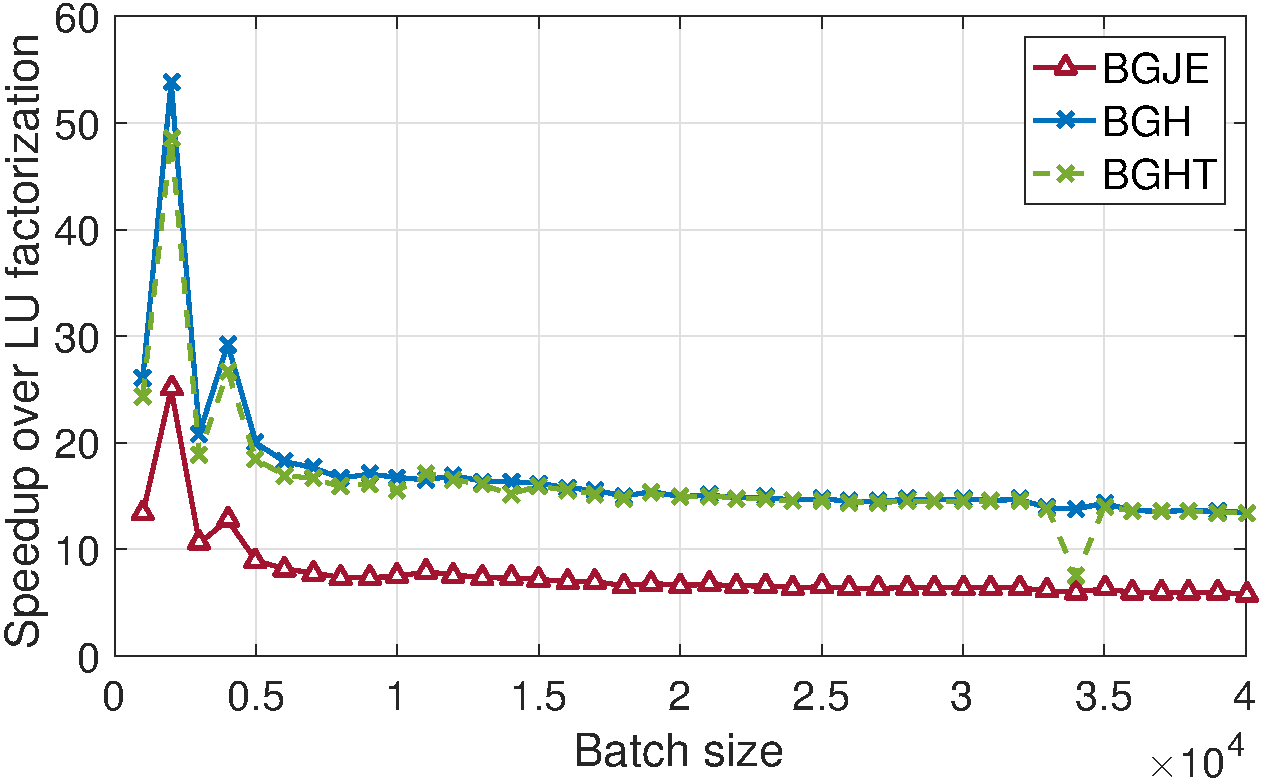
\includegraphics[width=.45\columnwidth]{plots/dgebjp_setup_P100_lu_gje_gh_16_speedup.pdf}
&
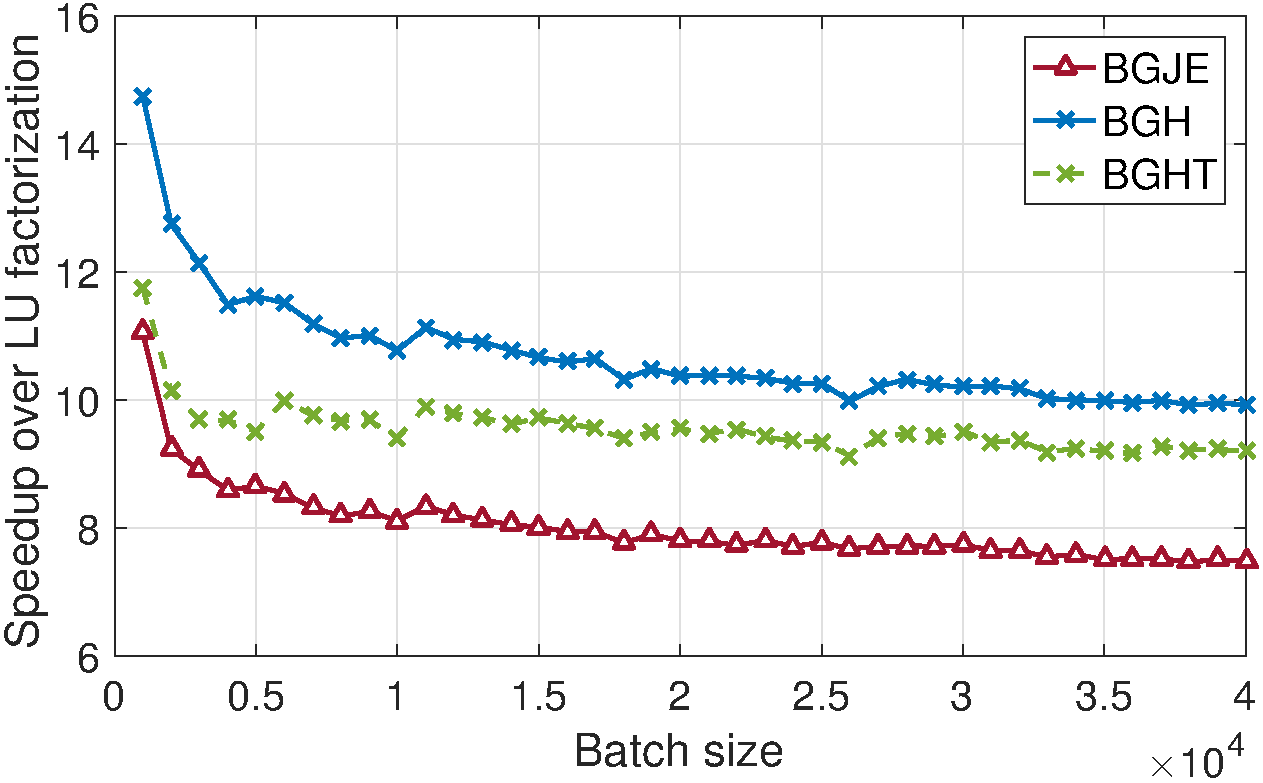
\includegraphics[width=.45\columnwidth]{plots/dgebjp_setup_P100_lu_gje_gh_32_speedup.pdf}
\end{tabular}
\end{center}
\caption{
Speedup of BGJE and BGH / BGHT over BLU taken from the MAGMA software package.
}
\label{2017-gh-block-jacobi:fig:bgjeperformance}
\end{figure}

\subsection{Performance of BGH}
Figure~\ref{2017-gh-block-jacobi:fig:bgjeperformance} compares the performance of our BGH implementation with 
alternative approaches providing similar functionality.
The baseline implementation is the batched LU factorization (BLU) kernel provided in the MAGMA library (version 2.0~\cite{magma}), designed for the LU factorization of a large set of small problems. We note that, conversely to the BGJE and BGH kernels,
the scope of the BLU kernel is limited to settings where all small systems are of the same same size. 
The results in the figure are expressed in terms of speedup over this routine.
BGJE is the implementation proposed in~\cite{gje}
which explicitly generates a block-inverse for Jacobi preconditioning.
For GH, we also include data for the variant storing the upper triangular part transposed (BGHT),
allowing for faster access during the preconditioner application.
As BLU currently only supports batches of equal-size problems, 
while BGJE and BGH only work for  problems of order up to 32,
we limit the analysis to block sizes 16 and 32.

For block size 16 (see left plot in Figure~\ref{2017-gh-block-jacobi:fig:bgjeperformance})
and large batch counts, the BGJE kernel is about 6$\times$ faster than BLU;
and we observe even larger speedups for smaller batch sizes.
Adding the transposed storage to the BGH kernel has a minor impact:
for relevant batch sizes, 
both BGH and BGHT are 
12--20$\times$ faster than BLU.
This is different for block size 32 (see right-hand side plot in Figure~\ref{2017-gh-block-jacobi:fig:bgjeperformance}):
Adding the transposed storage to the BGH kernel reduces 
the speedup of BGHT over BLU to values around 8.5$\times$, but
BGH remains more than 10$\times$ faster than BLU.
Even though BGJE computes the explicit inverse, 
and hence executes more operations than BLU and GH,
this kernel is more than 7.5$\times$ faster than BLU. 
For completeness, we mention that for block size 32, BGJE delivers
about 600 GFLOPS (billions of flops/second) on this architecture (see~\cite{gje}).



\begin{figure}
\begin{center}
\begin{tabular}{ll}
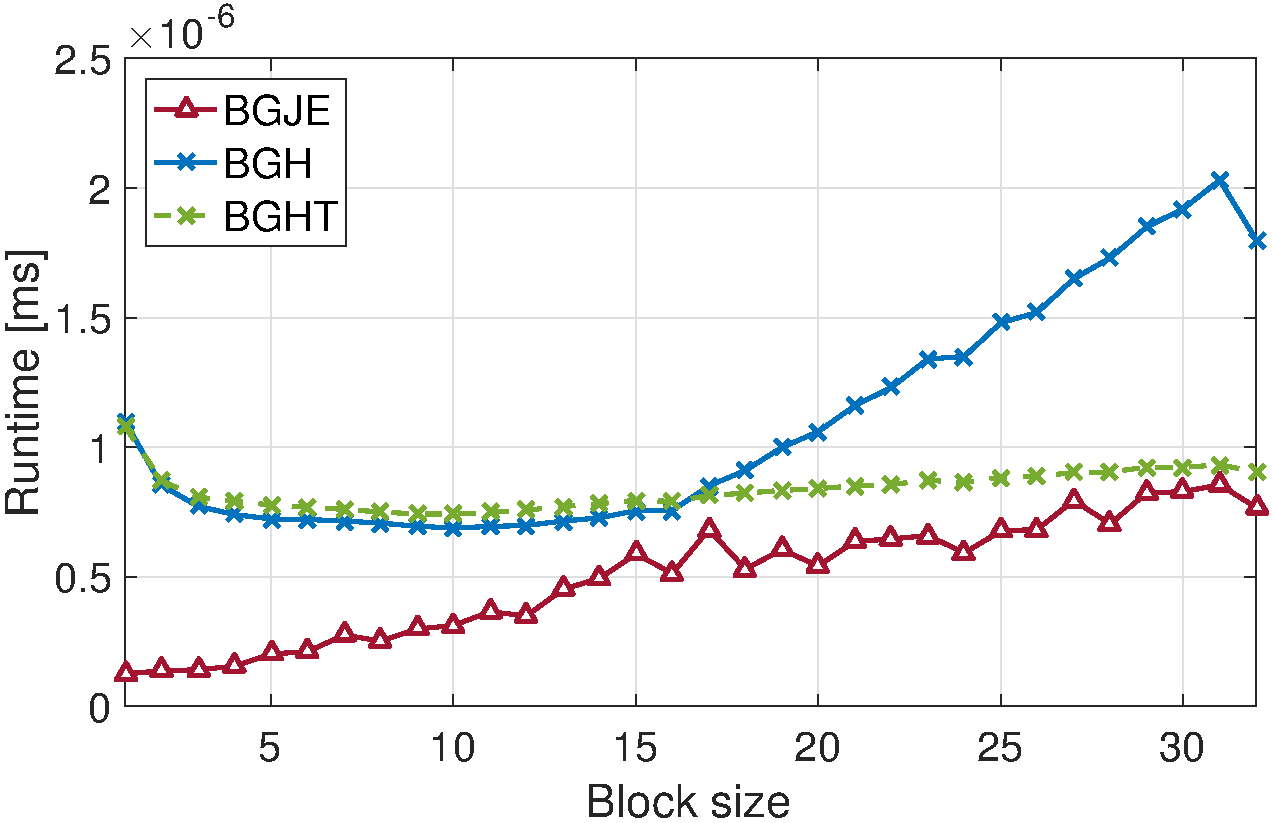
\includegraphics[width=.45\columnwidth]{plots/app_dgebjp_setup_P100_spmv_gh_ght_apply_fixed.pdf}
&
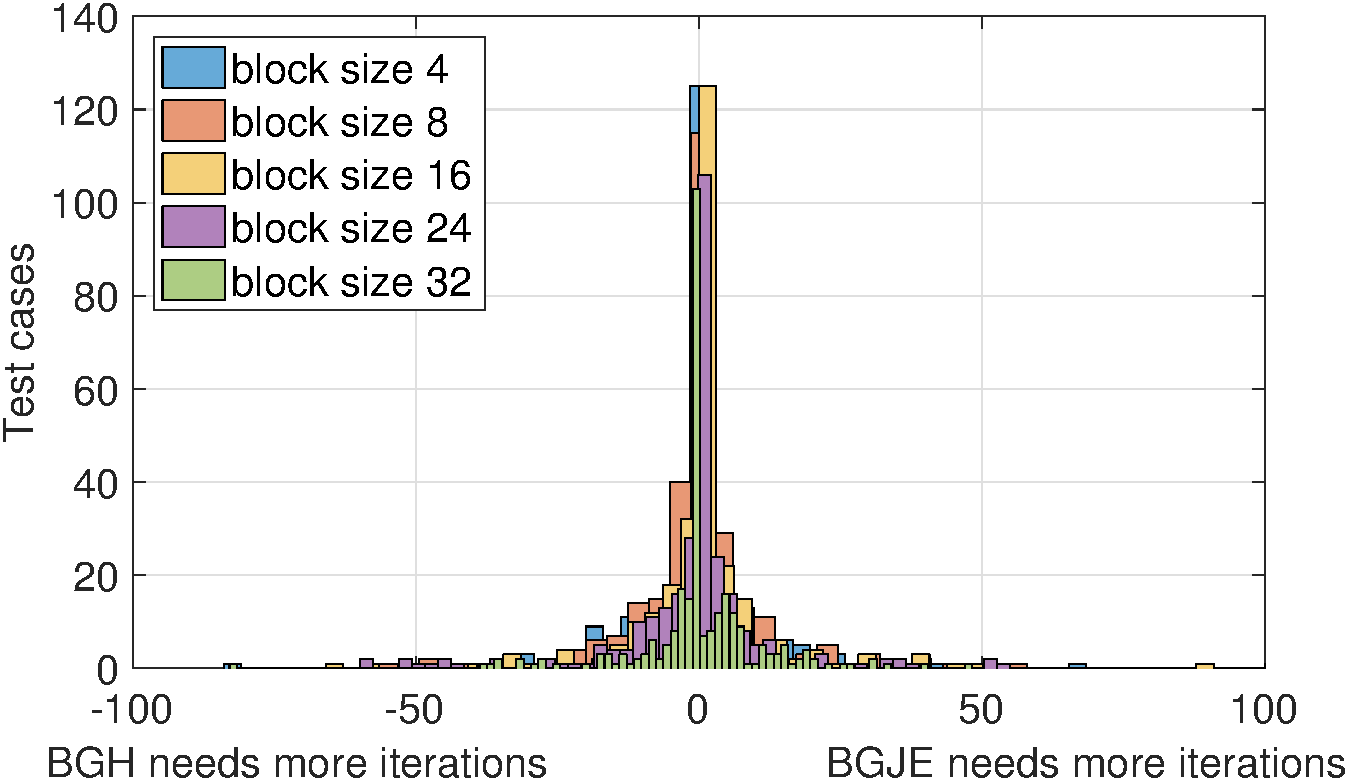
\includegraphics[width=.49\columnwidth]{plots/iteration_distribution}\\
\end{tabular}
\end{center}
\caption{
Left: Runtime of block-Jacobi application for distinct block sizes and a problem of row size 1,000,000.
Right: BiCGSTAB convergence variations when using block-Jacobi based on 
BGJE or BGH.
}
\label{2017-gh-block-jacobi:fig:app_performance}
\end{figure}



\subsection{Performance of block-Jacobi application}
Figure~\ref{2017-gh-block-jacobi:fig:app_performance} (left) shows the runtime
of three preconditioner application strategies:
sparse matrix-vector multiplication if the preconditioner was generated using GJE (BGJE),
versus Gauss-Huard application using diagonal blocks $\widetilde{D}_i$ (BGH)
or $\hat{D}_i$ (BGHT).
We fix the problem size to 1~million rows and consider different diagonal block sizes.
As could be expected, the approach based on the sparse matrix-vector product 
is always faster than both GH-based application strategies,
which can be attributed to the lower number of flops
and better workload balance.

Even though half of the memory accesses in BGH are noncoalescent,
we observe only minor performance deviations from the BGHT kernel for block sizes smaller than 16.
An explanation is that smaller blocks fit into less cache lines,
so they can be read only once,
and kept in cache for the duration of the kernel.
If this happens, the noncoalescent reads are as fast as the coalescent ones,
and both strategies result in the same performance.
Once the blocks become too large for cache, some cache lines need to be evicted
during the GH application, and noncoalescent reads in BGH start to impact the performance
of this approach.

\begin{figure*}
\begin{center}
\begin{tabular}{lr}
\hline
Block size 16\\
\begin{adjustbox}{valign=t}
  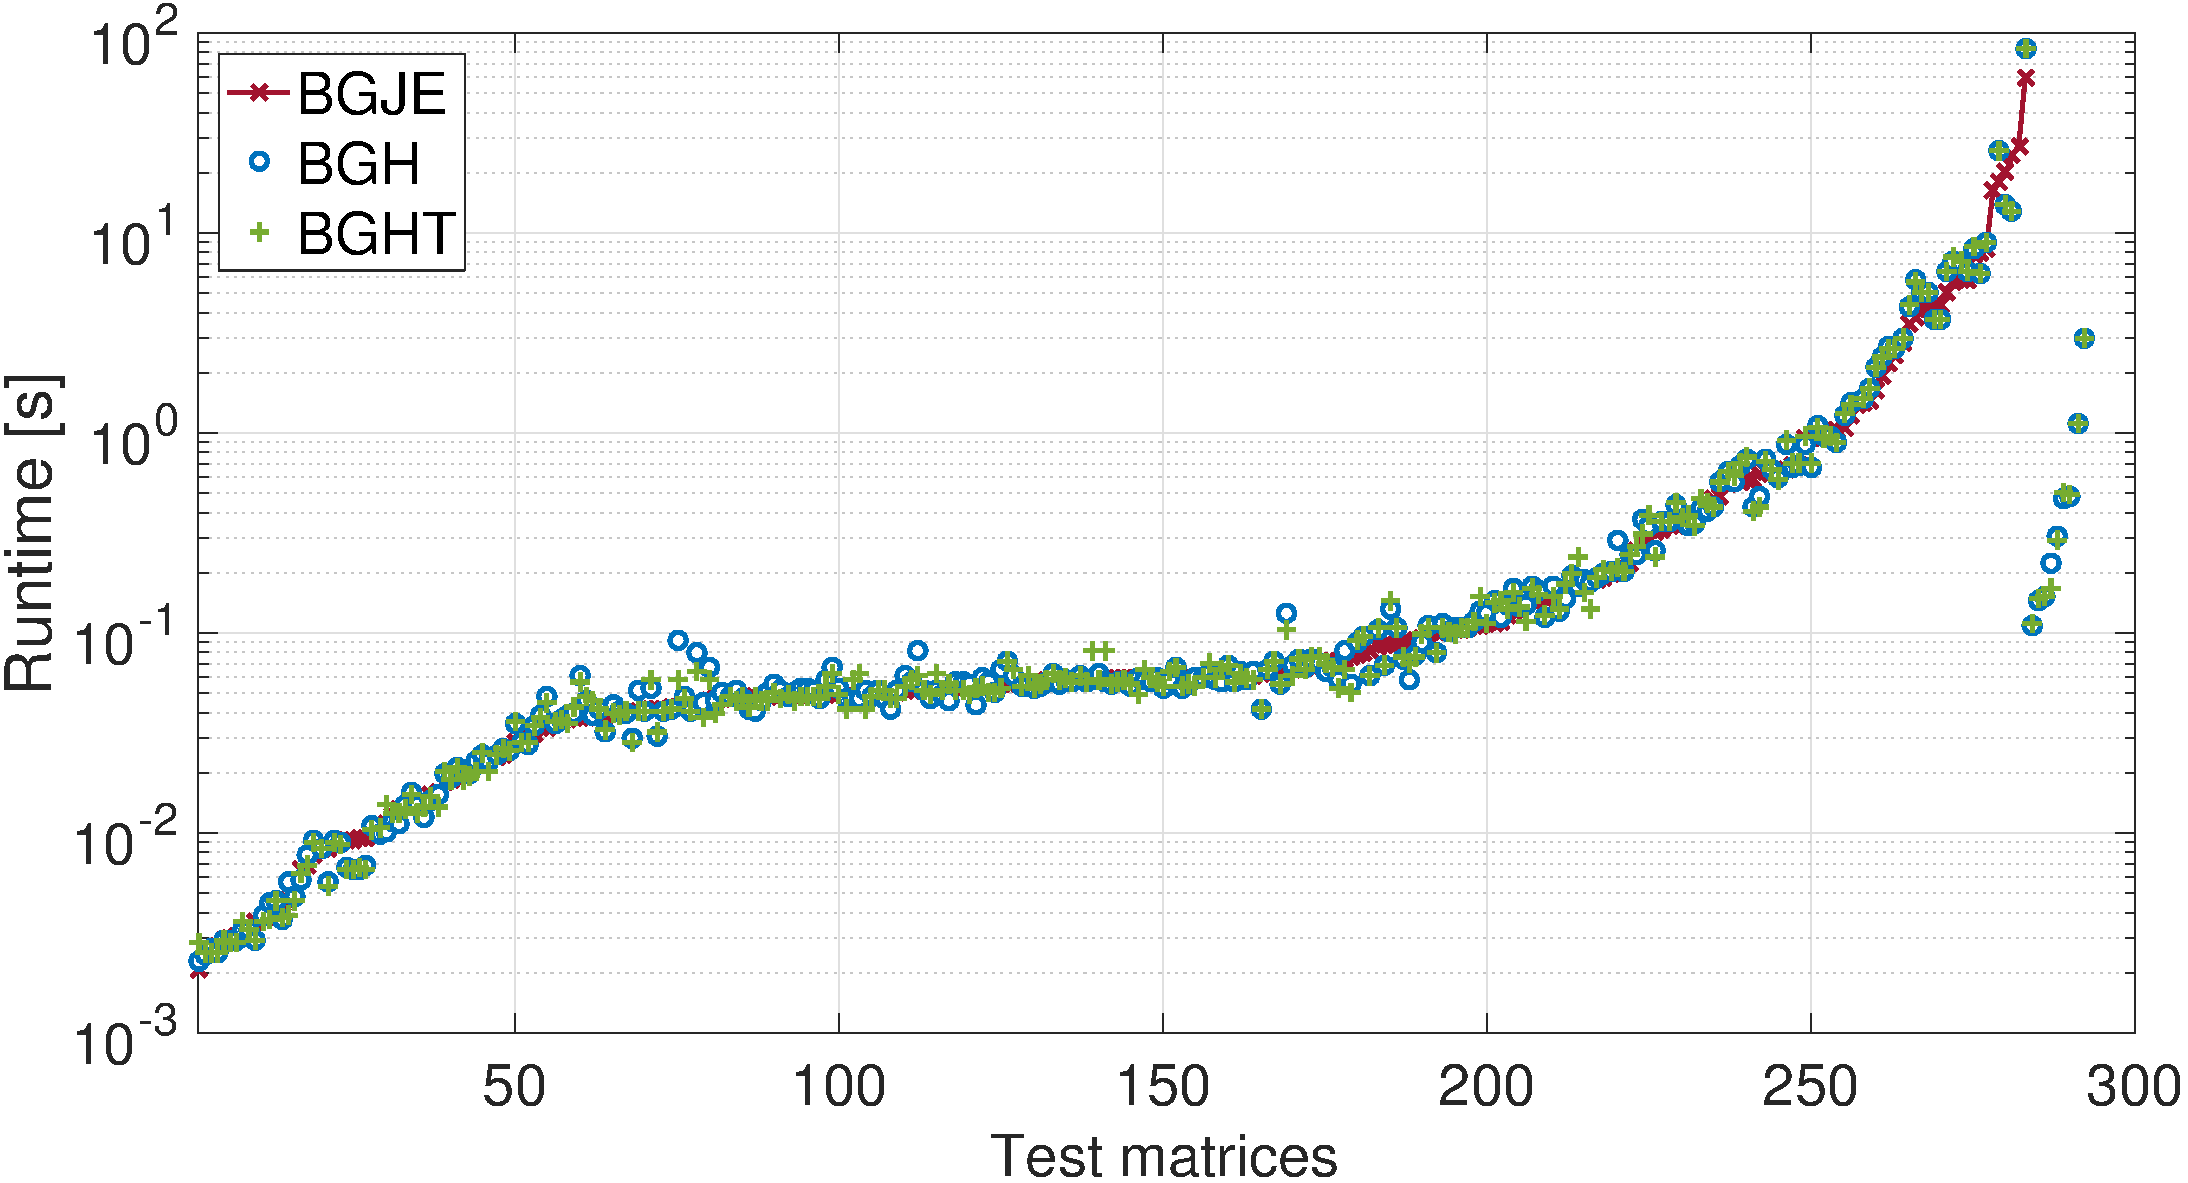
\includegraphics[width=.65\columnwidth]{plots/runtime_comparison_bs16.pdf}
\end{adjustbox}
&
\begin{adjustbox}{valign=t}
    \begin{tabular}{@{}c@{}}
        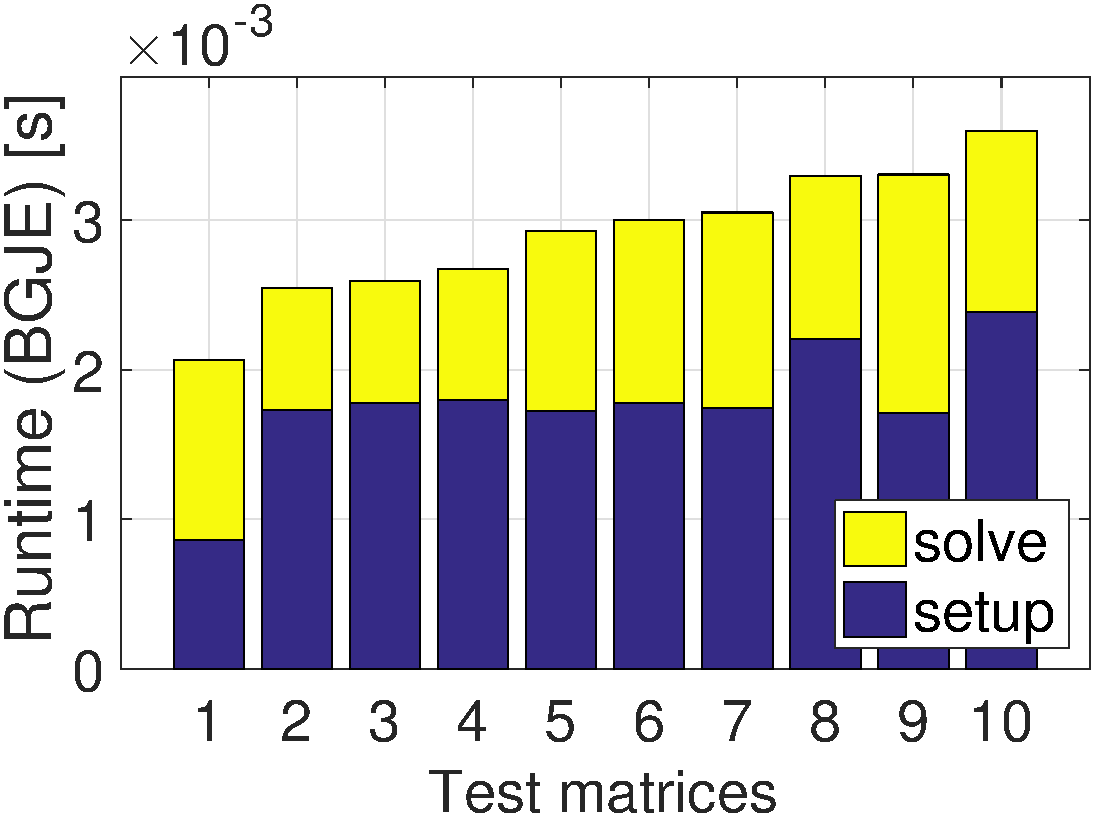
\includegraphics[width=.27\columnwidth]{plots/barplot_bs16_GJE}\\[-3.65ex]
        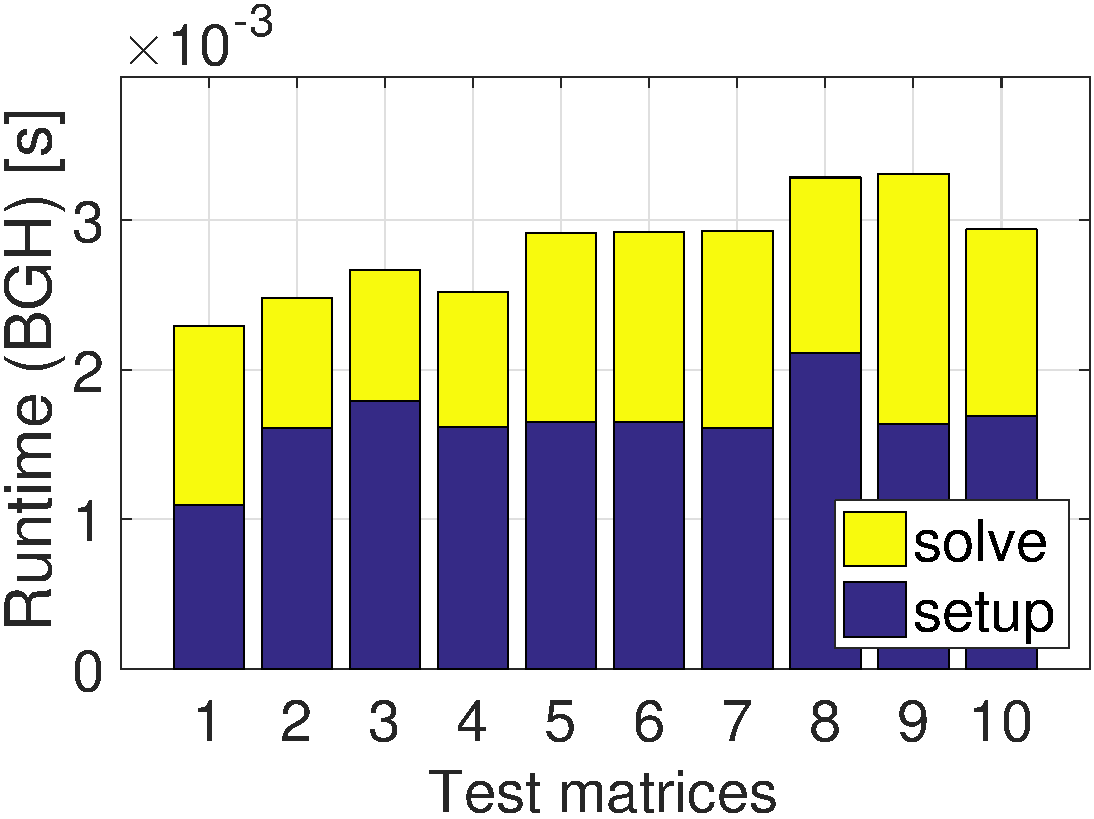
\includegraphics[width=.27\columnwidth]{plots/barplot_bs16_GH}
    \end{tabular}
\end{adjustbox}

\\
\hline
Block size 32\\
\begin{adjustbox}{valign=t}
  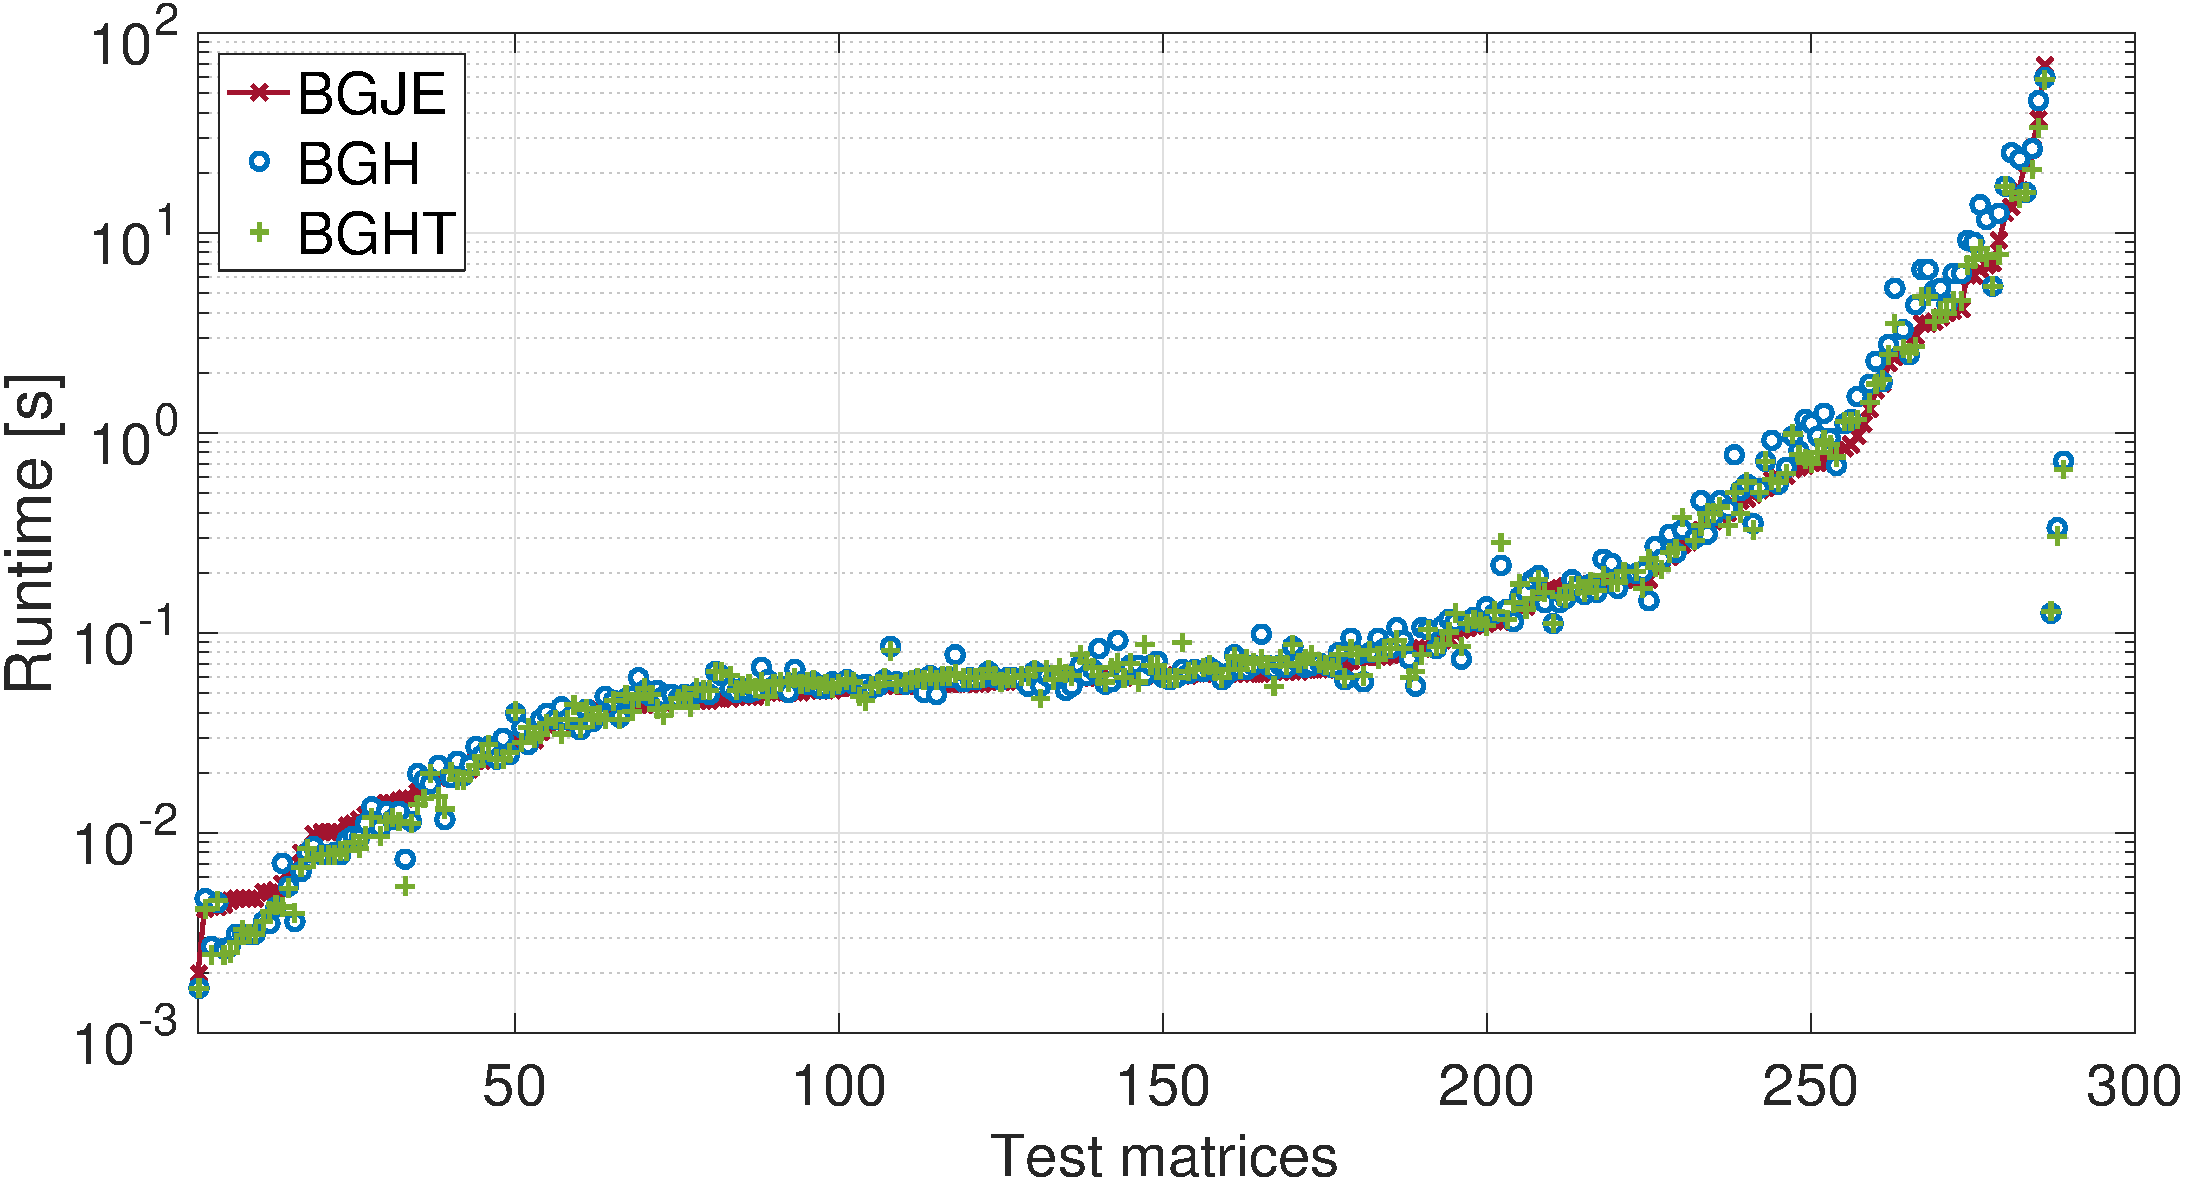
\includegraphics[width=.65\columnwidth]{plots/runtime_comparison_bs32.pdf}
\end{adjustbox}
&
\begin{adjustbox}{valign=t}
    \begin{tabular}{@{}c@{}}
        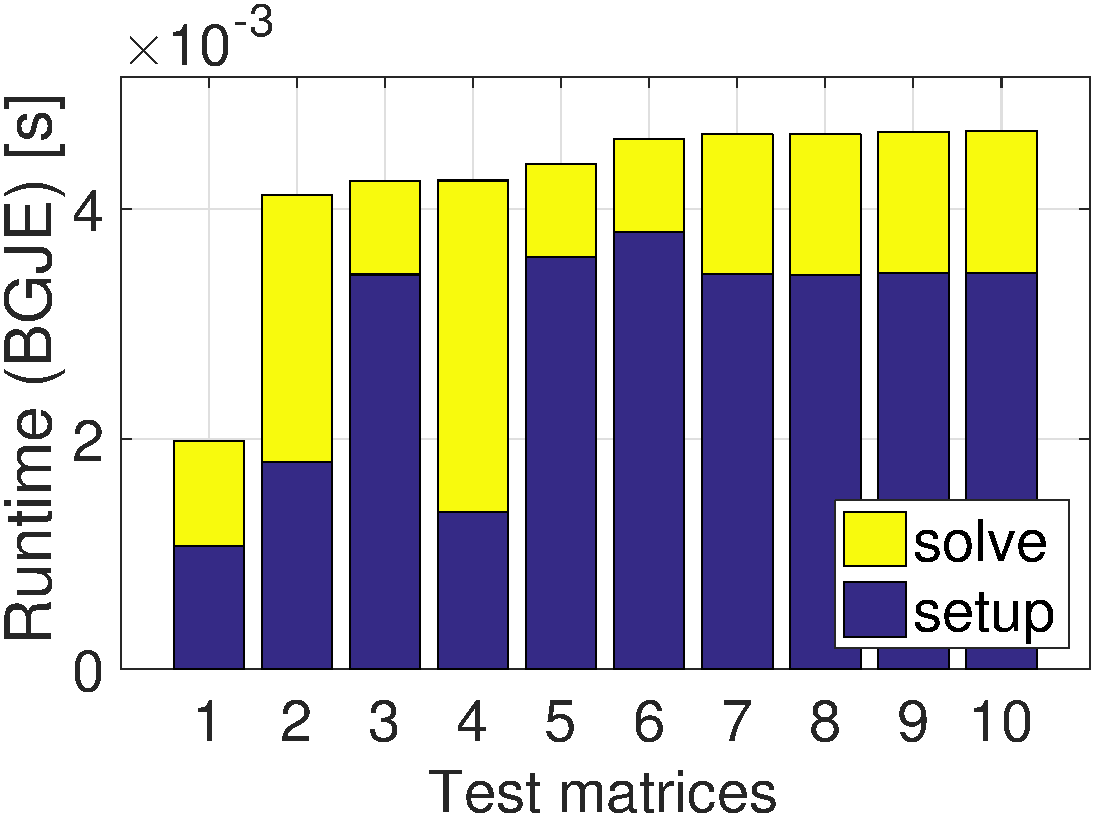
\includegraphics[width=.27\columnwidth]{plots/barplot_bs32_GJE}\\[-3.65ex]
        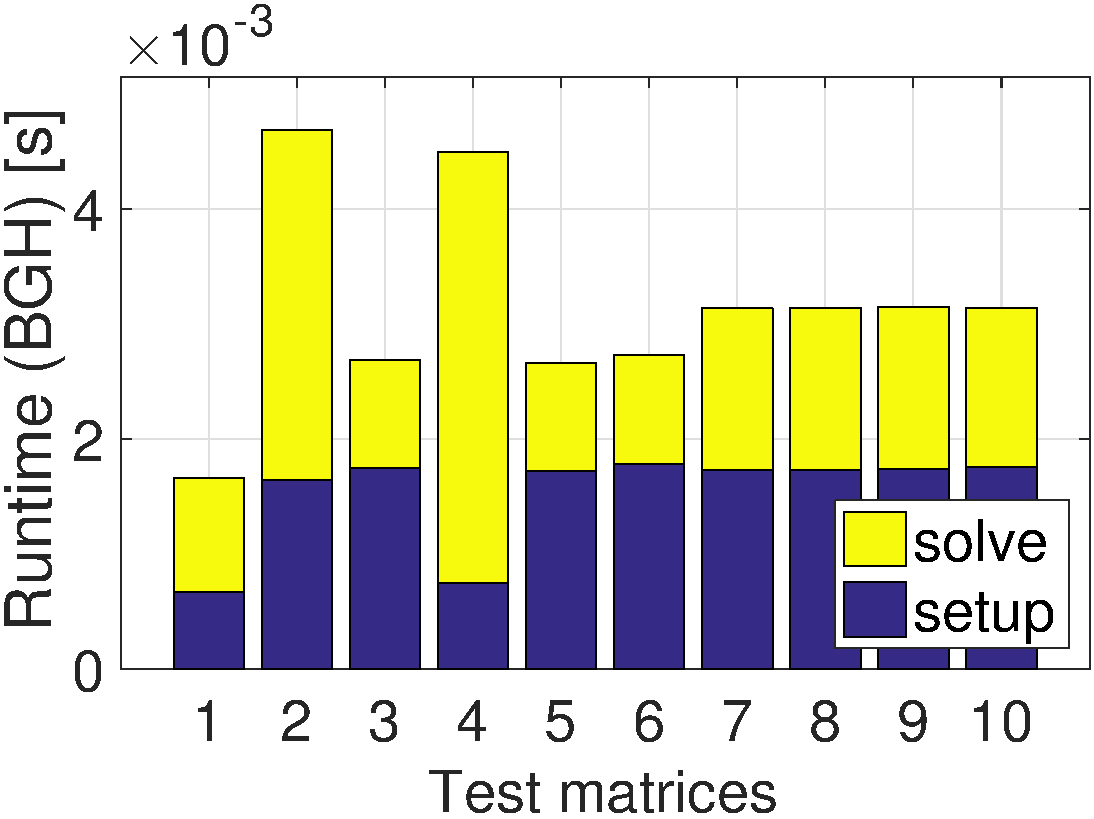
\includegraphics[width=.27\columnwidth]{plots/barplot_bs32_GH}
    \end{tabular}
\end{adjustbox}

\end{tabular}
\end{center}
\caption{
Left: Total execution time (setup+solve) 
for BiCGSTAB enhanced with block-Jacobi preconditioning based on either
BGJE, BGH or BGHT.
Top-level results are for a block-size bound 16; bottom-level results are for a block-size bound 32. 
Right: Decomposition of the total execution time into preconditioner setup time and iterative solver runtime
for the left-most test cases.
}
\label{2017-gh-block-jacobi:fig:block-jacobi-runtime}
\end{figure*}

\subsection{Iterative solver analysis}
We next assess the efficiency of the distinct strategies for block-Jacobi preconditioning in
an iterative solver framework. For this purpose we integrate 
the block-Jacobi preconditioner(s)
into the BiCGSTAB iterative solver provided
in MAGMA-sparse~\cite{ashes2016},
and test the preconditioned 
solver setting for a variety of linear systems. 
The test matrices are chosen from the SuiteSparse matrix collection~\cite{ufmc},
combined with a right-hand side vector with all entries equal to one. 
We start the iterative solver with an initial guess of zero,
and stop once the relative residual norm is decreased by six orders of magnitude.
We allow for up to 10,000 iterations. 

First, we evaluate whether the difference between GJE and GH in terms of numerical stability 
has any impact on the preconditioner efficiency. 
At this point, we recognize that rounding can have significant effect on
a preconditioner's efficiency,
and a more accurate preconditioner does not inevitably result in
faster convergence of the iterative solver. 
Figure~\ref{2017-gh-block-jacobi:fig:app_performance} (right)
displays the convergence difference
of BiCGSTAB depending on 
whether the block-Jacobi preconditioner is based 
on GH or GJE. 
The x-axis of the histogram reflects the iteration overhead;
the y-axis shows the number of test cases for which 
GJE provided a ``better'' preconditioner (bars left of center) or
GH did (bars right of center).
For all block sizes, the majority of the problems is located in the center,
reflecting the cases where both methods resulted in the same iteration count.
Furthermore, the histogram exposes a high level of symmetry,
suggesting that the numerical stability of the method based on explicit inversion plays a minor role.

While being similar from the convergence rate point of view, the pending question is
whether there exist any performance differences making GJE or GH superior.
The plot in the left-hand side of Figure~\ref{2017-gh-block-jacobi:fig:block-jacobi-runtime}
arranges the test systems according to increasing 
execution time of the BiCGSTAB solver preconditioned with block-Jacobi based on BGJE. 
The block structure was generated via the supervariable blocking routine
provided by MAGMA-sparse with a maximum block size of 16 (top) and 32 (bottom).
The execution times comprise both the preconditioner setup and the iterative solver times.
In addition to the block-Jacobi using BGJE, we also include the total solver runtime 
for the variants using BGH and BGHT.

In most cases, the BGH and BGHT execution times are close, or even match those of BGJE.
In particular for block size 32, 
the results may suggest that BGJE is slightly better if the execution time is large (right-most data).
Conversely, BGH and BGHT are faster if the solution time is small (left-most data).
On the right of Figure~\ref{2017-gh-block-jacobi:fig:block-jacobi-runtime} we decompose the total solution time 
into its preconditioner setup and iterative solver components for the first 10~test problems.
For these instances, the preconditioner setup time accounts for a significant portion
of the total solver execution time, and the higher cost of explicit block-inversion
is not compensated for by the slightly faster preconditioner application.
